\section{Program Logistics}

% Request review from Katy Huff
\subsection{Potential Speakers}

\subsubsection{Rachel Slaybaugh, UC Berkeley}
\begin{wrapfigure}{r}{0.5\textwidth}
	\begin{center}
		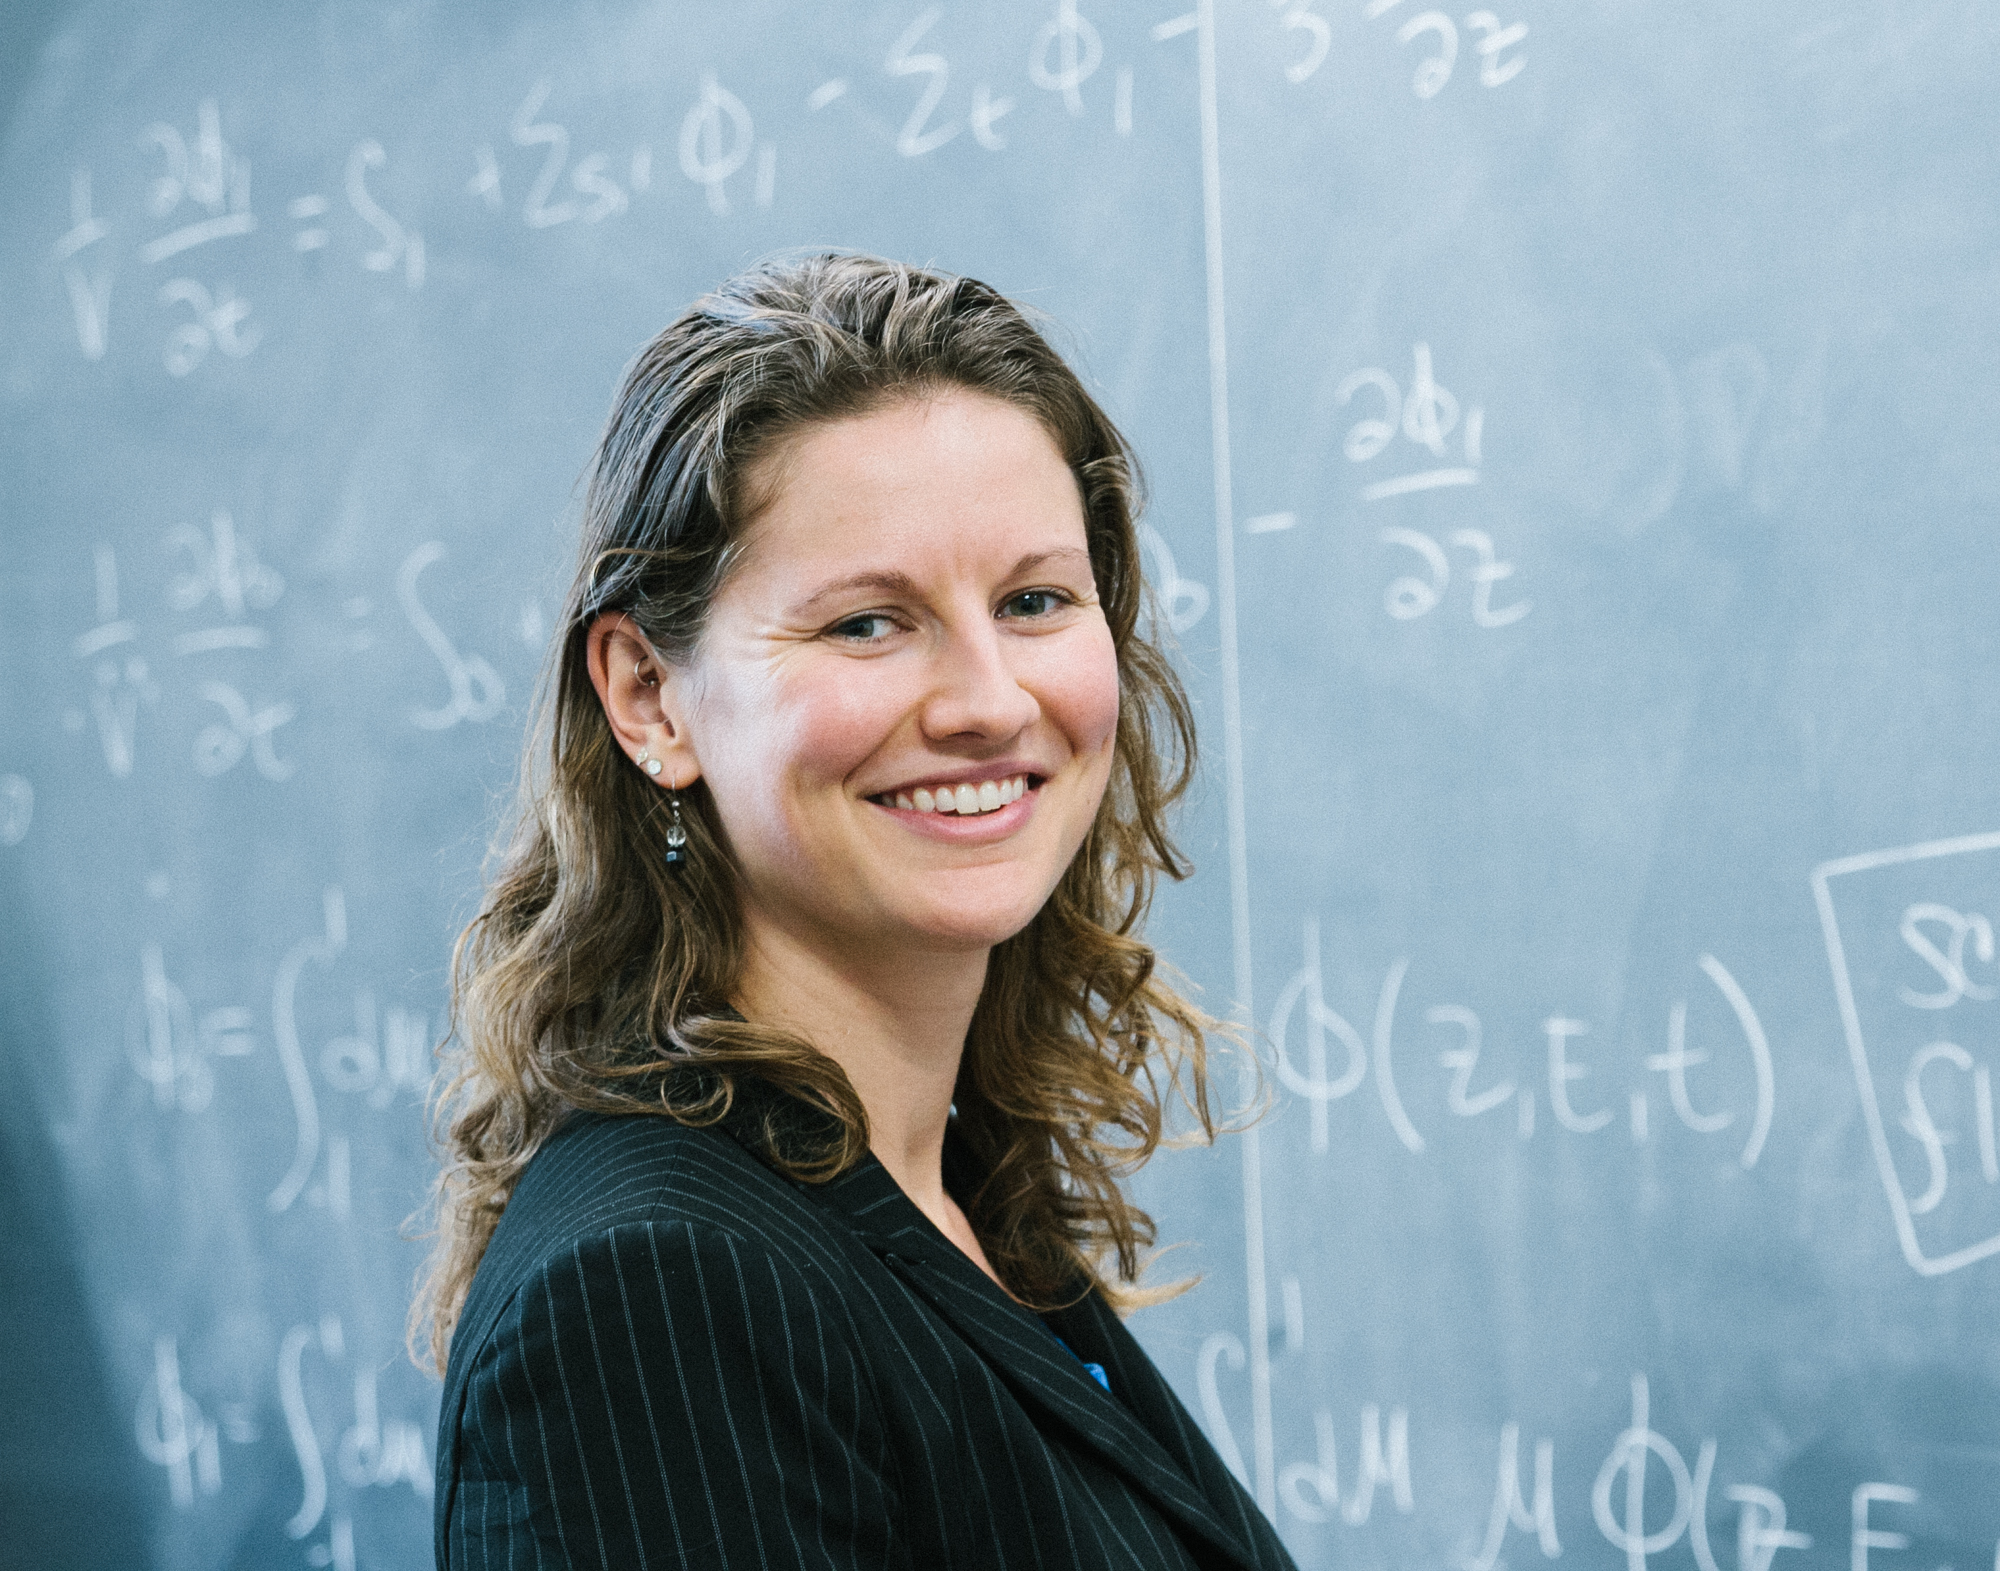
\includegraphics[width=0.48\textwidth,scale=0.2]{slaybaugh.jpg}
	\end{center}
\end{wrapfigure}
Prof. Slaybaugh's research is based in numerical methods for neutron transport with an emphasis on supercomputing. She applies these methods to reactor design, shielding, and nuclear security and nonproliferation. Slaybaugh was a key founder of the nuclear innovation bootcamp, which seeks to train students and professionals in skills essential to innovation in nuclear energy while executing team projects. Finally, Slaybaugh has served as a Program Director at ARPA-E, developing and running their first fission energy programs. Advanced Research Projects Agency-Energy (ARPA-E) invests in research for ways to generate, use, and store energy. These projects have the potential to radically improve economic prosperity in the U.S. and environmental wellbeing. Due to her endeavors in teaching and sharing nuclear innovation, we believe that Slaybaugh's goals are aligned with the goals of this conference and would make her an excellent addition to the program. Slaybaugh has much to offer the conference with her vision and leadership.
\subsubsection{Suzanne Hobbs Baker}
\begin{wrapfigure}{r}{0.5\textwidth}
	\begin{center}
		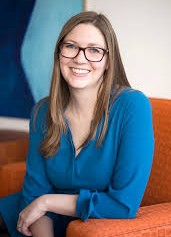
\includegraphics[scale=0.75]{hobbsbaker.jpeg}
	\end{center}
\end{wrapfigure}
Talking about nuclear energy, specifically with the general public, is one of Suzanne Hobbs Baker's key goals. Baker has a strong track record as a nuclear science communicator. In 2008 she founded a nonprofit organization aimed at reaching women, minorities, and young people with critical information about climate change and nuclear energy. She currently works as the creative director for Fast Path to Zero Initiatve at the University of Michigan and as a Nuclear security fellow with Third Way Energy. Baker's work in empowering minorities and students to solve the world climate crisis with nuclear energy, as well as her skill in creative science communication, ensures that Baker has a lot to offer the student conference. Celebrating the people behind the science is one of the key goals of this conference and an area in which Baker has a lot of experience.
\vfill
\subsubsection{Todd Allen, UW Madison}
\begin{wrapfigure}{r}{0.5\textwidth}
	\begin{center}
		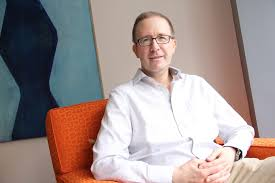
\includegraphics[scale=0.75,width=0.48\textwidth]{allen.jpeg}
	\end{center}
\end{wrapfigure}
His first post-Ph.D. position was as a staff scientist at Argonne National Laboratory. While at Argonne, he joined the leadership team tasked with developing the Generation IV Roadmap, the document that framed the resurgence of the nuclear research programs early in the 21st Century.Following Argonne, he joined the faculty at the University of Wisconsin. While there, he split his time between establishing a premier material science program at the university and supporting the Idaho National Laboratory. At INL, he led the transition of the Advanced Test Reactor into a national user facility. He also ran a six-institution Energy Frontier Research Center focused on answering fundamental questions about heat transfer in nuclear fuel.
From 2013-2016, he helped lead the Idaho National Laboratory as the Deputy Laboratory Director for Science $\&$ Technology, including being an important contributor to the development of the Gateway for Accelerated Innovation in Nuclear (GAIN) initiative announced at the White House in November 2015. Since 2016 he has been a Visiting Senior Fellow with Clean Energy Program at Third Way, a Washington, DC based think tank. His role in formulating the roadmap for Generation IV reactors and his leadership indicate that he would make a great speaker at the conference.
\subsubsection{Rita Baranwal, DOE Nuclear Energy}
\subsubsection{Jim Conca, Forbes}
\subsubsection{Fatima Ebrahimi, Princeton}


\subsection{Panels}

